\documentclass[]{tufte-handout}

% ams
\usepackage{amssymb,amsmath}

\usepackage{ifxetex,ifluatex}
\usepackage{fixltx2e} % provides \textsubscript
\ifnum 0\ifxetex 1\fi\ifluatex 1\fi=0 % if pdftex
  \usepackage[T1]{fontenc}
  \usepackage[utf8]{inputenc}
\else % if luatex or xelatex
  \makeatletter
  \@ifpackageloaded{fontspec}{}{\usepackage{fontspec}}
  \makeatother
  \defaultfontfeatures{Ligatures=TeX,Scale=MatchLowercase}
  \makeatletter
  \@ifpackageloaded{soul}{
     \renewcommand\allcapsspacing[1]{{\addfontfeature{LetterSpace=15}#1}}
     \renewcommand\smallcapsspacing[1]{{\addfontfeature{LetterSpace=10}#1}}
   }{}
  \makeatother
\fi

% graphix
\usepackage{graphicx}
\setkeys{Gin}{width=\linewidth,totalheight=\textheight,keepaspectratio}

% booktabs
\usepackage{booktabs}

% url
\usepackage{url}

% hyperref
\usepackage{hyperref}

% units.
\usepackage{units}


\setcounter{secnumdepth}{-1}

% citations

% pandoc syntax highlighting
\usepackage{color}
\usepackage{fancyvrb}
\newcommand{\VerbBar}{|}
\newcommand{\VERB}{\Verb[commandchars=\\\{\}]}
\DefineVerbatimEnvironment{Highlighting}{Verbatim}{commandchars=\\\{\}}
% Add ',fontsize=\small' for more characters per line
\newenvironment{Shaded}{}{}
\newcommand{\KeywordTok}[1]{\textcolor[rgb]{0.00,0.44,0.13}{\textbf{{#1}}}}
\newcommand{\DataTypeTok}[1]{\textcolor[rgb]{0.56,0.13,0.00}{{#1}}}
\newcommand{\DecValTok}[1]{\textcolor[rgb]{0.25,0.63,0.44}{{#1}}}
\newcommand{\BaseNTok}[1]{\textcolor[rgb]{0.25,0.63,0.44}{{#1}}}
\newcommand{\FloatTok}[1]{\textcolor[rgb]{0.25,0.63,0.44}{{#1}}}
\newcommand{\ConstantTok}[1]{\textcolor[rgb]{0.53,0.00,0.00}{{#1}}}
\newcommand{\CharTok}[1]{\textcolor[rgb]{0.25,0.44,0.63}{{#1}}}
\newcommand{\SpecialCharTok}[1]{\textcolor[rgb]{0.25,0.44,0.63}{{#1}}}
\newcommand{\StringTok}[1]{\textcolor[rgb]{0.25,0.44,0.63}{{#1}}}
\newcommand{\VerbatimStringTok}[1]{\textcolor[rgb]{0.25,0.44,0.63}{{#1}}}
\newcommand{\SpecialStringTok}[1]{\textcolor[rgb]{0.73,0.40,0.53}{{#1}}}
\newcommand{\ImportTok}[1]{{#1}}
\newcommand{\CommentTok}[1]{\textcolor[rgb]{0.38,0.63,0.69}{\textit{{#1}}}}
\newcommand{\DocumentationTok}[1]{\textcolor[rgb]{0.73,0.13,0.13}{\textit{{#1}}}}
\newcommand{\AnnotationTok}[1]{\textcolor[rgb]{0.38,0.63,0.69}{\textbf{\textit{{#1}}}}}
\newcommand{\CommentVarTok}[1]{\textcolor[rgb]{0.38,0.63,0.69}{\textbf{\textit{{#1}}}}}
\newcommand{\OtherTok}[1]{\textcolor[rgb]{0.00,0.44,0.13}{{#1}}}
\newcommand{\FunctionTok}[1]{\textcolor[rgb]{0.02,0.16,0.49}{{#1}}}
\newcommand{\VariableTok}[1]{\textcolor[rgb]{0.10,0.09,0.49}{{#1}}}
\newcommand{\ControlFlowTok}[1]{\textcolor[rgb]{0.00,0.44,0.13}{\textbf{{#1}}}}
\newcommand{\OperatorTok}[1]{\textcolor[rgb]{0.40,0.40,0.40}{{#1}}}
\newcommand{\BuiltInTok}[1]{{#1}}
\newcommand{\ExtensionTok}[1]{{#1}}
\newcommand{\PreprocessorTok}[1]{\textcolor[rgb]{0.74,0.48,0.00}{{#1}}}
\newcommand{\AttributeTok}[1]{\textcolor[rgb]{0.49,0.56,0.16}{{#1}}}
\newcommand{\RegionMarkerTok}[1]{{#1}}
\newcommand{\InformationTok}[1]{\textcolor[rgb]{0.38,0.63,0.69}{\textbf{\textit{{#1}}}}}
\newcommand{\WarningTok}[1]{\textcolor[rgb]{0.38,0.63,0.69}{\textbf{\textit{{#1}}}}}
\newcommand{\AlertTok}[1]{\textcolor[rgb]{1.00,0.00,0.00}{\textbf{{#1}}}}
\newcommand{\ErrorTok}[1]{\textcolor[rgb]{1.00,0.00,0.00}{\textbf{{#1}}}}
\newcommand{\NormalTok}[1]{{#1}}

% longtable
\usepackage{longtable,booktabs}

% multiplecol
\usepackage{multicol}

% strikeout
\usepackage[normalem]{ulem}

% morefloats
\usepackage{morefloats}


% tightlist macro required by pandoc >= 1.14
\providecommand{\tightlist}{%
  \setlength{\itemsep}{0pt}\setlength{\parskip}{0pt}}

% title / author / date
\title{Scraping Nuclear Reactors}
\author{Data Computing}
\date{Computing Project}


\begin{document}

\maketitle




In this project, you're going to scrape data about nuclear reactors in
various courntries from Wikipedia.

\section{Tables in HTML pages}\label{tables-in-html-pages}

Go to the page
\url{http:://en.wikipedia.org/wiki/List_of_nuclear_reactors}. Find the
reactor list for Japan.

Although such lists are in a visual tabular format, they do not have a
simple data-table structure. The tables are organized using HTML tags,
which provide much more flexibility for visual appearance.

\begin{verbatim}
<table class="wikitable sortable">
<tr>
<th rowspan="2" style="background:#FFDEAD;">Name</th>
... and so on ...
</tr>
<tr>
<td>Fukushima Daiichi</td>
<td>1</td>
... and so on ...
</tr>
\end{verbatim}

Compare the human-readable version of the table with the HTML markup.
You'll see that the data is there, but there is a lot of extraneous
material and the arrangement is set not by position in a spreadsheet
layout but by \emph{HTML tags}\footnote{A markup indicator, analogous to
  \texttt{*} or \texttt{\#\#\#} or \texttt{{[}text{]}(line)} in
  markdown.} like \texttt{\textless{}td\textgreater{}} and
\texttt{\textless{}tr\textgreater{}}.

\subsection{Parsing HTML into a data
table}\label{parsing-html-into-a-data-table}

\enlargethispage{1in}

\begin{Shaded}
\begin{Highlighting}[]
\KeywordTok{library}\NormalTok{(rvest)}
\KeywordTok{library}\NormalTok{(lubridate)}
\NormalTok{page <-}\StringTok{ "http://en.wikipedia.org/wiki/List_of_nuclear_reactors"}
\NormalTok{table_nodes <-}\StringTok{ }\NormalTok{page %>%}
\StringTok{  }\KeywordTok{read_html}\NormalTok{() %>%}
\StringTok{  }\KeywordTok{html_nodes}\NormalTok{(}\StringTok{"table"}\NormalTok{)}
\NormalTok{table_list <-}
\StringTok{  }\KeywordTok{html_table}\NormalTok{(table_nodes[}\DecValTok{1}\NormalTok{:}\DecValTok{30}\NormalTok{], }\DataTypeTok{fill =} \OtherTok{TRUE}\NormalTok{)}
\end{Highlighting}
\end{Shaded}

The \texttt{table\_list} object is not quite a data table; it is a
\emph{list} of data tables. Here are some of the operations you can
apply to lists:

\begin{longtable}[]{@{}lll@{}}
\toprule
Description & Syntax & Example\tabularnewline
\midrule
\endhead
How many elements in the list & \texttt{length(}\emph{table}\texttt{)} &
\texttt{length(table\_list)}\tabularnewline
Grab a single element & \emph{table}\texttt{{[}{[}}\emph{element
number}\texttt{{]}{]}} &
\texttt{table\_list{[}{[}20{]}{]}}\tabularnewline
\bottomrule
\end{longtable}

\begin{enumerate}
\def\labelenumi{\arabic{enumi})}
\tightlist
\item
  Find the table element
\end{enumerate}

Start with \texttt{head(table\_list{[}{[}5{]}{]})} and go down the list
until you find the table for Japan. Keep in mind that the tables are
listed by number in the same order that they appear on the page. As of
the time of this writing,\footnote{Wikipedia articles are works in
  progress. Over a period of even a few days they may have been modified
  substantially.} \texttt{table\_list{[}{[}5{]}{]}} is for Austria, so
you'll have to go a good distance down the table to get to Japan.

\begin{verbatim}
table = table_list[[21]]  # change index for Japan
names(table)
\end{verbatim}

\begin{enumerate}
\def\labelenumi{\arabic{enumi})}
\setcounter{enumi}{1}
\tightlist
\item
  Look at it using \texttt{View()}
\end{enumerate}

The contents of row 1 don't refer to a case but to the variable names.
To clean this table, you will want to create meaningful variable names
and then delete row 1. You may need to refer to the original HTML
document to figure out what are appropriate names.

Here are some examples of the types of statements you might find helpful
for fixing the variable names.

\begin{Shaded}
\begin{Highlighting}[]
\NormalTok{new_names <-}\StringTok{ }\KeywordTok{c}\NormalTok{(}\StringTok{"first"}\NormalTok{, }\StringTok{"second"}\NormalTok{, }\StringTok{"third"}\NormalTok{)}
\KeywordTok{names}\NormalTok{(table) <-}\StringTok{ }\NormalTok{new_names }\CommentTok{# reset the variable names}
\NormalTok{table <-}\StringTok{ }\NormalTok{table[-}\DecValTok{1}\NormalTok{, ] }\CommentTok{# drop the first row}
\end{Highlighting}
\end{Shaded}

\subsection{A quick visualization}\label{a-quick-visualization}

\enlargethispage{1in}

\begin{marginfigure}
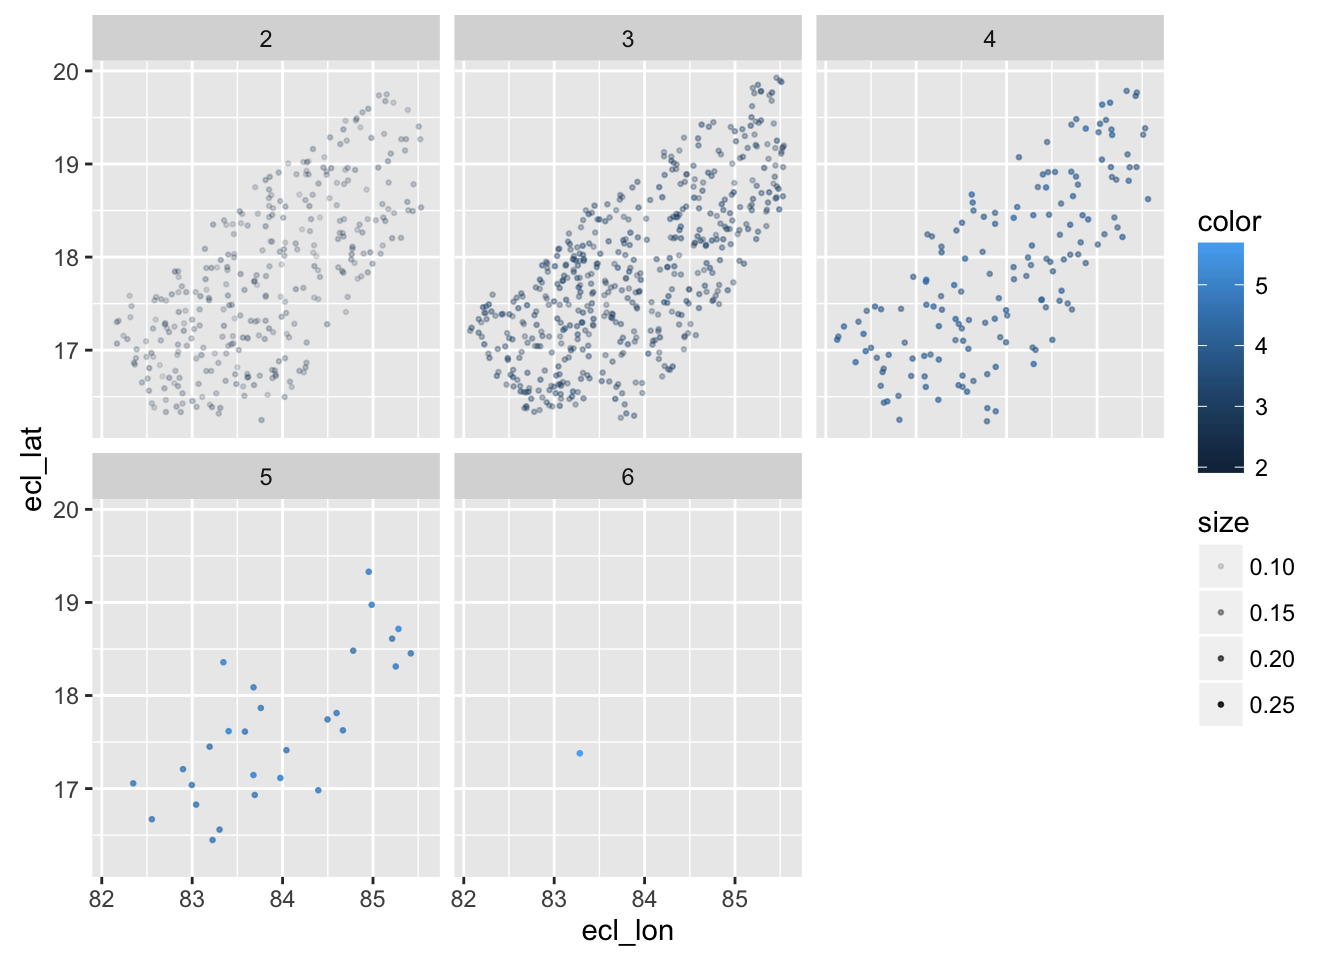
\includegraphics{832-NuclearReactors_files/figure-latex/unnamed-chunk-5-1} \end{marginfigure}

Plot out electrical capacity versus date of commissioning. Remember to
turn the commissioning date into a genuine \emph{date object}\footnote{A
  type of R object representing points in time but allowing plotting,
  extraction of components, and mathematical operations to be carried
  out.}. Color the points by the \emph{type} of reactor, e.g., BWR, PWR,
or FBR.\footnote{Boiling water reactor, pressurized water reactor, fast
  breeder reactor, respectively}

Interpretation: the net capacity of nuclear power plants in Japan tended
to increase over time (but then plateaued in recent years).

\subsection{Construction delays}\label{construction-delays}

Make an informative graphic that shows how long it took between start of
construction and commissioning for each nuclear reactor in Japan (or
another country of your choice). One possibility: use reactor name vs
date as the frame. For each reactor, set the glyph to be a line
extending from start of construction to commissioning. You can do this
with \texttt{geom\_segment()} using name as the y coordinate and time as
the x coordinate.

\begin{marginfigure}
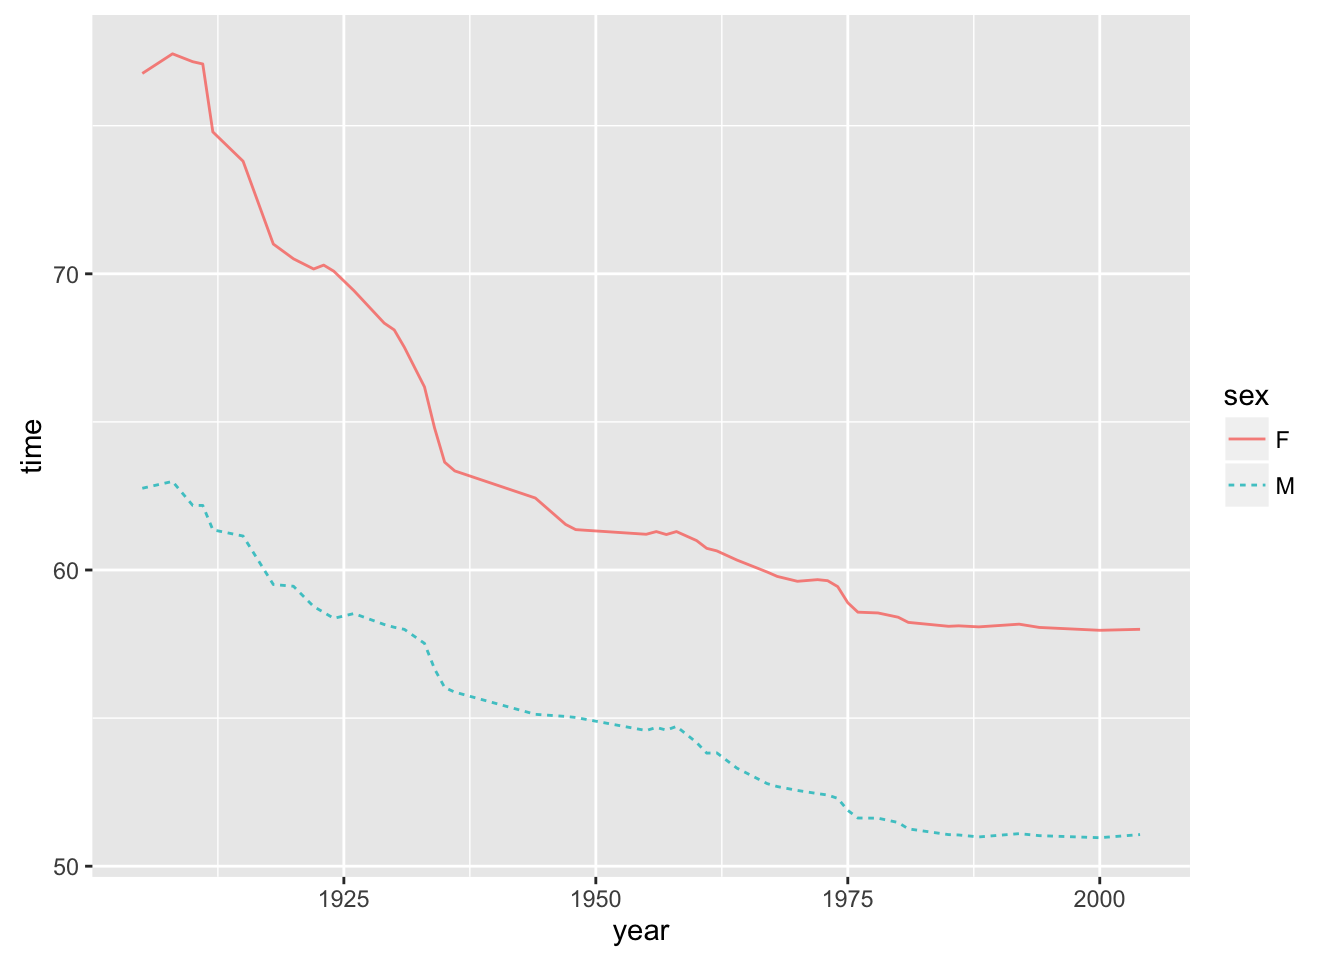
\includegraphics{832-NuclearReactors_files/figure-latex/unnamed-chunk-7-1} \end{marginfigure}



\end{document}
